%%%%%%%%%%%%%%%%%%%%%%%%%%%%%%%%%%%%%%%%%%%%%%%%%%%%%%%%%%
%%
%%  LOD-L4.tex
%%  Lecture 4: Generating Families, Dimension
%%
%%%%%%%%%%%%%%%%%%%%%%%%%%%%%%%%%%%%%%%%%%%%%%%%%%%%%%%%%%

\chapter*{\S L4. Generating Families, Dimension}
\setcounter{footnote}{0}

%%%%%%%%%%%%%%%%%%%%%%%%%%%%%%%%%%%%%%%%%%%%%%%%%%%%%%%%%%
%%
%% MARK: Abstract
%%
%%%%%%%%%%%%%%%%%%%%%%%%%%%%%%%%%%%%%%%%%%%%%%%%%%%%%%%%%%
\begin{abstract}
  In this lecture we introduce first the notion of \emph{generating family},
  and we'll see an application in the definition of \emph{dimension in diffeology}.
  Applied to the quotients $\Delta_m = \RR^m\!/\O(\RR^m)$,
  we prove that $\Delta_m$ and $\Delta_n$ are not diffeomorphic if $n \neq m$,
  and not diffeomorphic to the half-line $\Delta_\infty = \LeftClosedInterval{0,\infty} \subset \RR$.
\end{abstract}

%%%%%%%%%%%%%%%%%%%%%%%%%%%%%%%%%%%%%%%%%%%%%%%%%%%%%%%%%%
%%
%% MARK: Introduction
%%
%%%%%%%%%%%%%%%%%%%%%%%%%%%%%%%%%%%%%%%%%%%%%%%%%%%%%%%%%%

The notion of \emph{dimension} in diffeology,
that was introduced in \cite{PIZ07},
is a quick and easy answer to the question:
\emph{For two different integers $n$ and $m$,
are the diffeological spaces $\Delta_n = \RR^n\!/\O(n)$ and $\Delta_m = \RR^m\!/\O(m)$ diffeomorphic?}
We will show that since $\dim(\Delta_n) = n$ and since the
dimension is a diffeological invariant,
the answer is \emph{No, they are not}.
This method simplifies a partial result,
obtained in a more complicated way in \cite{Igl85},
stating that $\Delta_1$ and $\Delta_2$ are not diffeomorphic.
The half-line $\Delta_\infty = \LeftClosedInterval{0, \infty} \subset \RR$ is a similar example for which $\dim(\Delta_\infty) = \infty$.
Hence,
$\Delta_m$ is not diffeomorphic to the half-line $\Delta_\infty$ for any integer $m$.
Dimension is a simple but powerful diffeological invariant.

%%%%%%%%%%%%%%%%%%%%%%%%%%%%%%%%%%%%%%%%%%%%%%%%%%%%%%%%%%
%%
%% MARK:  Generating Families
%%
%%%%%%%%%%%%%%%%%%%%%%%%%%%%%%%%%%%%%%%%%%%%%%%%%%%%%%%%%%
\section{Generating families}

Diffeologies can be built by \emph{generating families}.
Any family of parametrizations of a set generates a diffeology.
Conversely,
any diffeology is generated by some set of parametrizations.
This mode of construction of diffeologies is very useful because it can reduce the analysis of the properties of a diffeological space to a subset of its plots,
hopefully smaller than the whole diffeology.
The definition of generating diffeology leads to the definition of the dimension of a diffeological space,
which is a first global invariant of the category \{Diffeology\}.
And this construction also leads to the introduction of important subcategories of diffeological spaces,
for example the category of manifolds,
or the category of orbifolds and others.

\begin{Article}{Proposition.}{}
  Let $\cF$ be a family of parametrizations of a set $X$.
  There exists a finest diffeology on $X$ containing $\cF$,
  it is called the \emph{diffeology generated by $\cF$}.
  It is denoted by $\gen{\cF}$.
  The family $\cF$ is said to be a \emph{generating family} of the diffeological space $(X,\gen{\cF})$ \cite{PIZ07}.
  It is the intersection of the diffeologies containing $\cF$
  $$%
    \gen{\cF} = \bigcap_{\cD \in \Difflg(X) \atop \cF \subset \cD} \cD.
    $$%
  Let $X$ be a diffeological space,
  the set of families generating $X$ will be denoted by $\Gen(X)$.
  
  \smuline{If the family $\cF$ covers $X$},
  that is,
  if for all $x \in X$ there exists a parametrization $F \in \cF$ such that $x = F(r)$,
  with $r \in \Domain(F)$,
  then a plot of $\gen{\cF}$ is any parametrization $P \colon U \to X$ such that:
  
  {\upshape($\clubsuit$)}  For all $r \in U$ there exists an open neighborhood $V \subset U$ of $r$,
  a parametrization $F \in \cF$,
  and a smooth parametrization $Q \colon V \to \Domain(F)$ such that $P \restriction V = F \circ Q$.
  
  \smuline{If the family $\cF$ does not cover $X$},
  the easiest way is to add the constant parametrizations
  $$%
    \hat x \colon \RR^0 \to X
    \quad \text{with} \quad
    \hat x(0) = x,
    $$%
  to $\cF$.
  That gives a family $\hat\cF$ that covers $X$ and
  $$%
    \gen{\cF} = \gen{\hat\cF}.
    $$%
  
  \uline{Note 1.}  The empty family $\varnothing$ generates the discrete family,
  $$%
    \gen{\varnothing} = \cD_\circ.
    $$%
  
  \uline{Note 2.}  The diffeology $\cD$ of a diffeological space $X$ belongs to $\Gen(X)$.
  Generating family is a projector:
  $$%
    \gen{\cD} = \cD
    $$%
  
  \uline{Note 3.}  Generating families is an increasing function of fineness
  $$%
    \cF \subset \cF' \quad \Rightarrow \quad \gen{\cF} \subset \gen{\cF'}.
    $$%
\end{Article}

\begin{Article}{Pushing forward families.}{}
  Let $X$ and $X'$ be two sets.
  Let $\cF$ be a family of parametrizations of $X$,
  and let $f : X \to X'$ be a map.
  
  The pushforward $f_*(\cF)$ of the family $\cF$ by $f$ is defined by
  $$%
    f_*(\cF) = \left\{ f \circ F \mid F \in \cF \right\}.
    $$%
  Then,
  the diffeology generated by the pushforward of the family $\cF$ by $f$ is the pushforward by $f$ of the diffeology generated by $\cF$,
  that is,
  $$%
    \gen{f_*(\cF)} = f_*(\gen{\cF}).
    $$%
  In particular,
  let $X$ and $X'$ be two diffeological spaces,
  and
  let $f : X \to X'$ be a subduction.
  The pushforward $f_*(\cF)$ of any generating family $\cF$ for $X$ is a generating family for $X'$.
\end{Article}

\begin{Article}{Pulling back families.}{}
  Let $X$ and $X'$ be two sets.
  Let $\cF'$ be a family of parametrizations of $X'$,
  and let $f : X \to X'$ be any map.
  Let us define the \emph{pullback of the family $\cF'$ by $f$} as the family $f^*(\cF)$ of parametrizations $F : U \to X$ satisfying the following property:
  \begin{itemize}
    \item[($\diamondsuit$)] Either $f\circ F$ is constant or there exists an element $F' : U' \to X'$ of $\cF'$,
    and a smooth parametrization $\pphi : U \to U'$,
    such that $F' \circ \pphi = f \circ F$.
  \end{itemize}
  Then,
  the diffeology generated by the pullback $f^*(\cF')$ is the pullback by $f$ of the diffeology generated by $\cF$,
  that is,
  $$%
    \gen{f^*(\cF')} = f^*(\gen{\cF'}).
    $$%
  In particular,
  let $X$ and $X'$ be two diffeological spaces,
  and let $f : X \to X'$ be an induction.
  The pullback $f^*(\cF')$ of any generating family $\cF'$ for $X'$ is a generating family for $X$.
  Unfortunately,
  compared with the pushforward of a family,
  pulling back a small generating family may lead to a huge family,
  almost as big as the diffeology itself.
  That will be the next example.
  
  \Note The choice of a generating family is relatively arbitrary.
  For example,
  the empty family is equivalent to the
  family of constant parametrizations.
  If the family $\cF'$ is empty,
  its pullback is not empty,
  but is the set of the parametrizations of $X$ with values in the preimages of points $f^{-1}(x')$,
  $x' \in X'$.
  This is not surprising since the pullback of the discrete diffeology is the sum of the preimages of points,
  equipped with the coarse diffeology.
\end{Article}

\begin{Article}{Example: Generating the half-line.}{}
  Let the half line $\LeftClosedInterval{0, \infty} \subset \RR$ be equipped with the subset diffeology of $\RR$.
  Let $\cF$ be the generating family of $\RR$ reduced to the identity,
  $\cF = \{\Id_{\RR}\}$.
  Then the pullback of the generating family $\cF$ by the inclusion $j \colon \LeftClosedInterval{0, \infty} \to \RR$ is the whole diffeology of $\LeftClosedInterval{0, \infty}$.
\end{Article}

\begin{proof}
  Indeed,
  the pullback $j^*(\{\Id_{\RR}\})$ is the set of parametrizations $F \colon U \to \LeftClosedInterval{0,\infty}$ such that $j \circ F$ is constant,
  or there exists an element $F' \in \{\Id_{\RR}\}$ and a smooth parametrization $\pphi : U \to \Domain(F')$ such that $j \circ F = F' \circ \pphi$.
  
  Thus,
  $F' = \Id_{\RR}$,
  $\Domain(F') = \RR$, and then $F = \pphi$.
  Therefore,
  $F$ is any smooth parametrization of $\RR$ with values in $\LeftClosedInterval{0,\infty}$,
  and $j^*(\{\Id_{\RR}\})$ is the whole diffeology of the half-line.
\end{proof}

%%%%%%%%%%%%%%%%%%%%%%%%%%%%%%%%%%%%%%%%%%%%%%%%%%%%%%%%%%
%%
%% MARK:  Dimension of a diffeology
%%
%%%%%%%%%%%%%%%%%%%%%%%%%%%%%%%%%%%%%%%%%%%%%%%%%%%%%%%%%%
\section{Dimension of a diffeology}

The \emph{global dimension} of a diffeology, or a diffeological space,
defined now is a diffeological invariant.
It will be refined later in a pointwise dimension map.

\begin{Article}{Dimension of a parametrization.}{}
  \label{Dimension-of-a-parametrization}
  Let $P$ be an $n$-parametrization of some set $X$,
  $n \in \NN$.
  We say that $n$ is the \emph{dimension} of $P$,
  and we denote it by $\dim(P)$.
  That is,
  $$%
    \forall P \in \Params(X), \ \dim(P) = n \ \Leftrightarrow
    \ P \in \Params_n(X).
    $$%
\end{Article}

\begin{Article}{Dimension of a family of parametrizations.}{}
  Let $X$ be a set and let $\cF$ be any family of parametrizations of $X$.
  We define the \emph{dimension} of $\cF$ as the supremum of the dimensions of its elements,
  $$%
    \dim(\cF) = \Sup \{ \dim(F) \mid F \in  \cF \}.
    $$%
  Note that $\dim(\cF)$ can be infinite if for all $n \in \NN$ there exists an element $F$ of $\cF$ such that $\dim(F) = n$.
  In this case we denote $\dim(\cF) = \infty$.
\end{Article}

\begin{Article}{Dimension of a diffeology.}{}
  Let $\cD$ be a diffeology.
  The \emph{dimension} of $\cD$ is defined as the infimum of the dimensions of its generating families:
  $$%
    \dim(\cD) = \inf \{ \dim(\cF) \mid  \langle \cF \,\rangle = \cD \}.
    $$%
  Let $X$ be a diffeological space and $\cD$ be its diffeology,
  we define the dimension of $X$ as the dimension of $\cD$:
  $$%
    \dim(X) = \dim(\cD) \in \NN \cup \{\infty\}.
    $$%
\end{Article}

\begin{Article}{Dimensions of Euclidean Domains.}{}
  \label{Dimensions-of-numerical-domains}
  The diffeological dimension of a Euclidean domain $U \subset \RR^n$,
  equipped with the standard diffeology,
  is equal to $n$:
  $$%
    \forall U \in \Domains(\RR^n), \quad \dim(U) = n.
    $$%
\end{Article}

\begin{proof}
  Let $\Id_U$ be the identity map of $U$.
  The singleton $\{\Id_U\}$ is a generating family of $U$,
  therefore,
  $\dim(U) \leq \dim \{\Id_U\}$.
  Since $\dim\{\Id_U\} = n$,
  $\dim(U) \leq n$.
  Now let us assume that $\dim(U) < n$.
  Then,
  there exists a generating family $\cF$ for $U$ such that $\dim(\cF) < n$.
  Since the identity map $\Id_U$ is a plot in $U$,
  it lifts locally at every point along some element of $\cF$.
  Thus,
  for any $r \in U$ there exists a neighborhood $V$ of $r$,
  a parametrization $F \colon W \to U$,
  element of $\cF$ (that is, $F \in \Cinfty(W,U)$) and a smooth map $Q \colon V \to W$,
  such that $\Id_U \restriction V = \Id_V = F \circ Q$.
  But $\dim(\cF) < n$ implies that $\dim(F)= \dim(W) <n$.
  Now,
  the rank of the linear tangent map $\Der(F \circ Q)$ is less or equal to $\dim(W) <n$,
  but $\Der(F \circ Q) = \Der(\Id_V) = \Id_{\RR^n}$,
  thus $\Rank(\Der(F \circ Q)) = \Rank(\Id_{\RR^n}) = n$.
  Therefore,
  there is no generating family $\cF$ of $U$ with $\dim(\cF) <n$,
  and $\dim(U) = n$.
\end{proof}

\begin{Article}{Dimension zero spaces are discrete.}
  A diffeological space has dimension zero if and only if it is discrete.
\end{Article}

\begin{proof} Let $X$ be a set equipped with the discrete diffeology.
  Any plot $P \colon U \to X$ is locally constant.
  Then,
  for any $r \in U$,
  $P$ lifts locally along the $0$-plot $\bmx = [0 \mapsto x]$,
  where $x = P(r)$.
  Hence,
  the $0$-plots form a generating family and $\dim(X) = 0$.
  Conversely,
  let $X$ be a diffeological space such that $\dim(X) = 0$.
  Then,
  the $0$-plots generate the diffeology of $X$.
  But,
  any plot lifting locally along a $0$-plot is locally constant.
  Therefore, $X$ is discrete.
\end{proof}

\begin{Article}{The dimension is a diffeological invariant.}{}
  \label{The-dimension-is-a-diffeological-invariant}
  If two diffeological spaces are diffeomorphic, then they have
  the same dimension.
\end{Article}

\begin{proof}
  Let $X$ and $X'$ be two diffeological spaces and let $f \in \Diff(X,X')$.
  Let $\cF$ be a generating family of $X$.
  The pushforward $\cF' = f_*(\cF)$ made of the plots $f \circ F$,
  where $F \in \cF$,
  is clearly a generating family of $X'$.
  Conversely we have $f^{-1}$.
  Therefore,
  $\dim(X) = \dim(X')$.
\end{proof}

\begin{Article}{Example: Has the set $\{0,1\}$ dimension 1?}{}
  Let us realize the set $\{0,1\}$ as the quotient of the real line $\RR$ by the projection
  $$%
    \left\{
    \begin{array}{l}
    \pi \colon \RR \to \{0,1\} \\
    \pi(x) = 0 \text{ if } x \in \QQ, \text{ and } \pi(x) = 1 \text{ otherwise.}
    \end{array}
    \right.
    $$%
  Let then $\{0,1\}_{\pi}$ be the set $\{0,1\}$ equipped with the diffeology generated by the parametrization $\pi$.
  Since $\{\pi\}$ is a generating family,
  the dimension of $\{0,1\}_\pi$ is less than or equal to $1 = \dim(\{\pi\})$.
  But,
  since the plot $\pi$ is not locally constant,
  by density of the rational (or irrational) numbers in $\RR$,
  the space $\{0,1\}_\pi$ is not discrete.
  Hence, $\dim\{0,1\}_\pi\neq 0$,
  and finally $\dim \{0,1\}_\pi = 1$.
  Thus,
  a finite diffeological space may have a non-zero dimension.
\end{Article}

\begin{Article}{Example: Dimension of tori.}{}
  Let $\Gamma \subset \RR$ be any strict subgroup of $(\RR,+)$ and let $\Torus_\Gamma$ be the quotient $\RR/\Gamma$,
  whose diffeology is generated by the projection  $\Class \colon \RR \to \RR/\Gamma$.
  Then,
  $$%
    \dim(\Torus_\Gamma) = 1.
    $$%
  This applies in particular to the circles $\RR/a \ZZ$,
  with perimeter $a > 0$,
  or to \emph{irrational tori} when $\Gamma$ is generated by more than one generator,
  rationally independent.
\end{Article}

\begin{proof}
  Since $\RR$ is a Euclidean domain,
  $\Class$ is a plot of the quotient,
  and $\cF = \{\Class\}$ is a generating family of $\RR/\Gamma$,
  and $\dim(\cF) = 1$.
  Thus,
  as a direct consequence of the definition
  $\dim(\RR/\Gamma) \leq 1$.
  Now,
  if $\dim(\RR/\Gamma) = 0$,
  then the diffeology of the quotient is generated by the constant parametrizations.
  But $\pi$ is not locally constant,
  therefore $\dim(\RR/\Gamma) = 1$.
\end{proof}

%%%%%%%%%%%%%%%%%%%%%%%%%%%%%%%%%%%%%%%%%%%%%%%%%%%%%%%%%%
%%
%% MARK:  Dimension Map of a Diffeological Space
%%
%%%%%%%%%%%%%%%%%%%%%%%%%%%%%%%%%%%%%%%%%%%%%%%%%%%%%%%%%%
\section{Dimension map of a diffeological space}

Because diffeological spaces are not necessarily homogeneous,
the global dimension of a diffeological space is a too rough invariant.
It is necessary to refine this definition and to introduce the dimension function of a diffeological space,
defined at each of its points.

The dimension function of diffeological spaces is the simplest numerical invariant in diffeology.

\begin{Article}{Pointed plots and germ of a diffeological space.}{}
  Let $X$ be a diffeological space,
  let $x \in X$.
  Let $P \colon U \to X$ be a plot.
  We say that $P$ is \emph{pointed at $x$} if $0 \in U$ and $P(0) = x$.
  We will agree that the set of \emph{germs} of the pointed plots of $X$ at $x$ represents the \emph{germ of the diffeology} at this point,
  and we shall denote it by $\cD_x$.
\end{Article}

\begin{Article}{Local generating families.}{}
  Let $X$ be a diffeological space and let $x$ be a point in $X$.
  We shall call \emph{local generating family at $x$} any family $\cF$ of plots of $X$ such that:
  
  \begin{enumerate}
    \item Every element $P$ of $\cF$ is pointed at $x$,
    that is,
    $0 \in \Domain(P)$ and $P(0) =x$.
    \item For all plots $P \colon U \to X$ pointed at $x$,
    there exists a neighborhood $V$ of $0 \in U$,
    a parametrization $F \colon W \to X$ belonging to $\cF$ and a smooth parametrization $Q \colon V \to W$ pointed at $0\in W$,
    such that $F \circ Q = P \restriction V$.
  \end{enumerate}
  
  We shall say also that $\cF$ \emph{generates the germ} $\cD_x$ of the diffeology $\cD$ of $X$ at the point $x$.
  And we denote
  $$%
    \cD_x = \langle \cF \rangle.
    $$%
  Note that,
  for any $x$ in $X$,
  the set of local generating families at $x$ is not empty,
  since it contains the set of all the plots pointed at $x$,
  and this set contains the constant parametrizations with value $x$.
\end{Article}

\begin{Article}{Local generating families.}{}
  Let $X$ be a diffeological space.
  Let us choose,
  for every $x \in {X}$,
  a local generating family $\cF_x$ at $x$.
  The union $\cF$ of all these local generating families,
  $$%
    \cF = \bigcup_{x \in {X}}\cF_x,
    $$%
  is a generating family of the diffeology of $X$.
\end{Article}

\begin{proof}
  Let $P \colon U \to X$ be a plot,
  let $r \in U$ and $x = P(r)$.
  Let $T_r$ be the translation $T_r(r') = r' + r$.
  Let $P' = P \circ T_r$ defined on $U' = T_r^{-1}(U)$.
  Since the translations are smooth,
  the parametrization $P'$ is a plot of $X$.
  Moreover $P'$ is pointed at $x$,
  $P'(0) = P \circ T_r (0) = P(r) = x$.
  By definition of a local generating family,
  there exists an element $F \colon W \to X$ of $\cF_x$,
  a neighborhood $V'$ of $0 \in U'$ and a smooth parametrization $Q' : V' \to W$,
  pointed at $0$,
  such that $P' \restriction V' = F \circ Q'$.
  Thus,
  $P \circ T_r \restriction V' = F \circ Q'$,
  that is,
  $P \restriction V = F \circ Q$,
  where $V = T_r(V')$ and $Q = Q' \circ T_r^{-1}$.
  Hence,
  $P$ lifts locally,
  at every point of its domain,
  along an element of $\cF$.
  Therefore,
  $\cF$ is a generating family of the diffeology of $X$.
\end{proof}

\begin{Article}{The dimension map.}{}
  Let $X$ be a diffeological space and let $x$ be a point of $X$.
  By analogy with the global dimension of $X$,
  we define the \emph{dimension of $X$ at the point $x$} by:
  $$%
    \dim_x(X) = \inf \{ \dim(\cF) \mid \langle \cF \rangle = \cD_x \}.
    $$%
  The map $x \mapsto \dim_x(X)$,
  with values in $\NN \cup \{\infty\}$,
  is called the \emph{dimension map} of the space $X$.
\end{Article}

\begin{Article}{Global dimension and dimension map.}{}
  Let $X$ be a diffeological space.
  The global dimension of $X$ is the supremum of the dimension map of $X$:
  $$%
    \dim(X) = \Sup_{x \in X} \{\dim_x(X)\}.
    $$%
\end{Article}

\begin{proof} Let $\cD$ be the diffeology of $X$.
  Let us prove first that for every $x \in X$, $\dim_x(X) \leq \dim(X)$,
  which implies that $\Sup_{x \in X} \dim_x(X) \leq \dim(X)$.
  For that we shall prove that for any $x \in X$ and any generating family $\cF$ of $\cD$,
  $\dim_x(X) \leq \dim(\cF)$.
  Then,
  since $\dim(X) = \inf \{ \dim(\cF) \mid \cF \in \cD \text{ and } \langle \cF \rangle = \cD \}$ we shall get,
  $\dim_x(X) \leq \dim(X)$.
  
  Now,
  let $\cF$ be a generating family of $\cD$.
  For any plot $P \colon U \to X$ pointed at $x$,
  let us choose an element $F$ of $\cF$ such that:
  there exists a neighborhood $V$ of $0 \in U$ and a smooth parametrization $Q : V \to {\rm def}(F)$,
  such that $F \circ Q = P \restriction V$.
  
  Then,
  let $r = Q(0)$ and $T_r$ be the translation $T_r(r') = r' + r$.
  Let $F' = F \circ T_r$,
  defined on $T_r^{-1}({\rm def}(F))$.
  
  Thus,
  $F'(0) = x$,
  and $F'$ is a plot of $X$,
  pointed at $x$,
  such that $\dim(F') = \dim(F)$.
  Let $Q' = T_r^{-1} \circ Q$,
  then $Q'$ is smooth and $P \restriction V = F' \circ Q'$.
  
  Thus,
  the set $\cF'_x$ of all these plots $F'$ associated with the plots pointed at $x$ is a generating family of $\cD_x$,
  and for each of them $\dim(F') = \dim(F) \leq \dim(\cF)$.
  
  Hence,
  $\dim(\cF'_x) \leq \dim(\cF)$.
  But $\dim_x(X) \leq \dim(\cF'_x)$,
  thus $\dim_x(X) \leq \dim(\cF)$.
  And we conclude that $\dim_x(X) \leq \dim(X)$,
  for any $x \in X$,
  and $\Sup_{x \in X} \dim_x(X) \leq \dim(X)$.
  
  Next,
  let us prove that $\dim(X) \leq \Sup_{x \in X} \dim_x(X)$.
  Let us assume that $\Sup_{x \in X} \dim_x(X)$ is finite.
  Otherwise,
  according to the
  previous part we have $\Sup_{x \in X} \dim_x(X) \leq \dim(X)$,
  and then $\dim(X)$ is infinite and $\Sup_{x \in X} \dim_x(X) = \dim(X)$.
  
  Now,
  for any $x \in X$,
  $\dim_x(X)$ is finite.
  And since the sequence of the dimensions of the generating families of $\cD_x$ is bounded below,
  there exists for any $x$ a generating family $\cF_x$ such that $\dim_x(X) = \dim(\cF_x)$.
  For every $x$ in $X$ let us choose one of them.
  
  Next,
  let us define $\cF_m$ as the union of all these chosen families.
  According to a proposition above,
  $\cF_m$ is a generating family of $\cD$.
  Hence, $\dim(X) \leq \dim(\cF_m)$.
  But $\dim(\cF_m) = \Sup_{F \in \cF_m} \dim(F) = \Sup_{x \in X} \Sup_{F \in \cF_x} \dim(F) = \Sup_{x \in X} \dim(\cF_x) = \Sup_{x \in X} \dim_x(X)$.
  
  Therefore,
  $\dim(X) \leq \Sup_{x \in X} \dim_x(X)$.
  And we can conclude,
  from the two parts above,
  that $\dim(X) = \Sup_{x \in X} \dim_x(X)$.
\end{proof}

\begin{Article}{The dimension map is a local invariant.}{}
  Let $X$ and $X'$ be two diffeological spaces.
  If $x \in X$ and $x' \in X'$ are two points related by a local (a fortiori global) diffeomorphism,
  then $\dim_x(X) = \dim_{x'}(X')$.
\end{Article}

\begin{Article}{Dimensions of manifolds.}{}
  An $n$-manifold is a diffeological space $X$ generated by local diffeomorphisms with $\RR^n$.
  Each such local diffeomorphism is called a \emph{chart} of $X$.
  Note that,
  each point is locally equivalent to any other point:
  there exists always a local diffeomorphism from one point to any other.
  The dimension function is constant,
  equal to the global dimension.
  Now,
  since there is always a chart mapping $0 \in \RR^n$ to $x \in X$,
  $\dim_x(X) = \dim_0(\RR^n)= n$.
  Therefore,
  $\dim(X) = n$.
  Which is coherent with the usual dimension in differential geometry.
\end{Article}

\begin{Article}{Klein decomposition.}{}
  Let $X$ be a diffeological space.
  The local diffeomorphisms of $X$ split the space into classes,
  according to the  relation:
  $x \sim x'$ if and only if there exists a local diffeomorphism $f$ mapping $x$ to $x'$.
  These classes are called the {\em orbits of the local diffeomorphisms} of $X$.
  We call these classes \emph{Klein orbits}.
  The dimension map is constant on each Klein orbit.
\end{Article}

%%%%%%%%%%%%%%%%%%%%%%%%%%%%%%%%%%%%%%%%%%%%%%%%%%%%%%%%%%
%%
%% MARK:  Examples of the half-lines
%%
%%%%%%%%%%%%%%%%%%%%%%%%%%%%%%%%%%%%%%%%%%%%%%%%%%%%%%%%%%
\section{Examples of the half-lines}

\begin{Article}{The half-line $\Delta_n$.}{}
  \label{Dimension-of-Rn/On}
  Let $\Delta_n = \RR^n/\O(n)$ equipped with the quotient diffeology,
  $n \in \NN$.
  Then,
  $\dim_0(\Delta_n) = n$,
  and $\dim_x(\Delta_n) = 1$ if $x \neq 0$.
  Thus, $\dim(\Delta_n) = n$ and for $n \neq m$ the half-lines $\Delta_n$ and $\Delta_m$ are not diffeomorphic.
\end{Article}

\begin{proof} Let $n>0$,
  and let us denote by $\Class_n : \RR^n \to \Delta_n$ the projection from $\RR^n$ onto its quotient.
  There is a natural bijection $f \colon \Delta_n \to \LeftClosedInterval{0,\infty}$ such that
  $$%
    f \circ \Class_n = \nu_n
    \quad \text{with} \quad
    \nu_n(x) = \Norm{x}^2.
    $$%
  Now, thanks to the uniqueness of quotients,
  we use $f$ to identify $\Delta_n$ with $\LeftClosedInterval{0,\infty}$,
  equipped with the diffeology $\cD_n$ generated by $\nu_n$.
  %
  \begin{center}
    \begin{tikzcd}[column sep=large, row sep=large, every label/.append style = {font = \small}]
      \RR^n \arrow[dr, "\nu_n"] \arrow[d, swap, "\pi_n"] &  {}  \\
      \Delta_n \arrow[r, swap, "f"] & \LeftClosedInterval{0,\infty}
    \end{tikzcd}
  \end{center}
  %
  The elements of $\cD_n$ consist of the parametrizations which can be lifted locally along $\nu_n$ by smooth parametrizations of $\RR^n$.
  Thus,
  since $\dim(\nu_n) = n$,
  we get $\dim(\Delta_n) \leq n$.
  Let us prove now that $\dim(\Delta_n) \geq n$:
  
  Let us assume that $\nu_n$,
  which is an element of $\cD_n$,
  can be lifted locally,
  at the point $0_n$,
  along a plot
  $$%
    P \in \cD_n \SpacedText{with} \dim(P) = p < n.
    $$%
  Then,
  there
  exists a smooth parametrization
  $$%
    \pphi : V \to \Domain(P)
    \quad \text{such that} \quad
    P \circ \pphi = \nu_n \restriction V.
    $$%
  We can assume without loss of generality that
  $$%
    0_p \in \Domain(P), \ P(0_p) = 0 \SpacedText{and} \pphi(0_n) = 0_p.
    $$%
  Now,
  since $P$ is an element of $\cD_n$,
  there exists a smooth parametrization
  $$%
    \psi \colon W \to \RR^n \SpacedText{such that} 0_p \in W \SpacedText{and} \nu_n \circ \psi = P \restriction W.
    $$%
  Let $V' = \pphi^{-1}(W)$,
  we get
  $$%
    \nu_n \restriction V' = \nu_n \circ F \SpacedText{with} F = \psi \circ \pphi \restriction V',
    $$%
  and
  $$%
    F \in \Cinfty(V', \RR^n), \ 0_n \in V' \SpacedText{and} F(0_n) = 0_n,
    $$%
  that is
  $$%
    \Norm{x}^2 = \Norm{F(x)}^2.
    $$%
  The second derivative of this
  identity computed at the point $0_n$ gives
  $$%
    \Id_n = M^t M \SpacedText{with} M = \Der(F)(0_n).
    $$%
  This is summarized by the following diagram:
  %
  \begin{center}
    \begin{tikzcd}[column sep=huge, row sep=2.5cm, every label/.append style = {font = \small}]
      {} & W \arrow[dr, "\psi"] \arrow[d, "P \restriction W" description] & {} \\
      V' \arrow[r,swap, "\nu_n \restriction V'"] \arrow[ur,"\pphi \restriction V'"] & \LeftClosedInterval{0,\infty} & \RR^n \arrow[l,"\nu_n"]
    \end{tikzcd}
  \end{center}
  %
  But
  $$%
    M = A B \SpacedText{with} A = \Der(\psi)(0_p) \SpacedText{and} B = \Der(\pphi)(0_n).
    $$%
  Thus,
  $\Id_n = B^tA^t A B$,
  which is impossible because $\Rank( B) \leq p < n$.
  Therefore,
  $\dim(\Delta_n) = n$.
  And,
  since the dimension is a diffeological invariant,
  $\Delta_n$ is not diffeomorphic to $\Delta_m$ for $n \neq m$.
\end{proof}

\begin{Article}{The half-line $\Delta_\infty$.}{}
  \label{Dimension-of-the-half-line}
  The dimension of a diffeological subspace $A \subset X$ can be less,
  equal,
  or even greater than the dimension of $X$.
  The following example is an illustration of this phenomenon.
  Let $\Delta_\infty = \LeftClosedInterval{0,\infty} \subset \RR$,
  equipped with the subset diffeology.
  Then,
  $$%
    \dim_0(\Delta_\infty) = \infty \SpacedText{and} \dim_x(\Delta_\infty) = 1 \SpacedText{if} x \neq 0.
    $$%
  Thus,
  $\dim(\Delta_\infty) = \infty$,
  and for any integer $m$,
  $\Delta_\infty$ is not diffeomorphic to $\Delta_m$.
\end{Article}

\begin{proof}
  Let us assume that $\dim(\Delta_\infty) = N < \infty$.
  For any integer $n$,
  the map $\nu_n : \RR^n \to \Delta_\infty$,
  defined by $\nu_n(x) = \Norm{x}^2$,
  belongs to $\cD_\infty$,
  the subset diffeology on $\LeftClosedInterval{0,\infty}$.
  %
  \begin{center}
    \begin{tikzcd}[column sep=large, row sep=1.5cm, every label/.append style = {font = \small}]
    {} & U \arrow[d,"f"] \\
    V\arrow[ur, "\pphi"] \arrow[r, swap, "\nu_n \restriction V"] & \LeftClosedInterval{0,\infty}    \\
    \end{tikzcd}
  \end{center}
  %
  Hence,
  $\nu_n$ lifts locally at the point $0_n$ along some $P \in \cD_\infty$,
  where $\dim(P) =p \leq N$.
  Now,
  let us choose $n > N$.
  Then,
  $P$ belongs to some $\Cinfty(U,\RR)$ with $\Val(P) \subset \LeftClosedInterval{0,\infty}$,
  and there exists a smooth parametrization $\pphi : V \to U$ such that $P \circ \pphi = \nu_n \restriction V$.
  We can assume,
  without loss of generality,
  that $0_p \in U$,
  $\pphi(0_n) = 0_p$,
  and thus:
  $P(0_p) = 0$.
  
  Now,
  the first derivative of $\nu_n$ at a
  point $x \in V' = \pphi^{-1}(V)$ is given by $x = \Der(P)(\pphi(x)) \circ \Der(\pphi)(x)$.
  But,
  since $P$ is smooth and positive,
  and since $P(0)=0$ we have $\Der(P)(0_p) = 0$.
  
  Hence,
  the second derivative of $\nu_n$ computed at the point $0_n$ gives $\Id_n = M^t H M$,
  where $M = \Der(\pphi)(0)$ and $H = \Der^2(P)(0)$.
  But since $\Rank(M) \leq p \leq N$ and  $n > N$,
  this is impossible,
  and the dimension of the embedded line is infinite at the origin,
  $\dim(\Delta_\infty) = \infty$.
\end{proof}

\begin{figure}[t]
  \vspace{\baselineskip}
  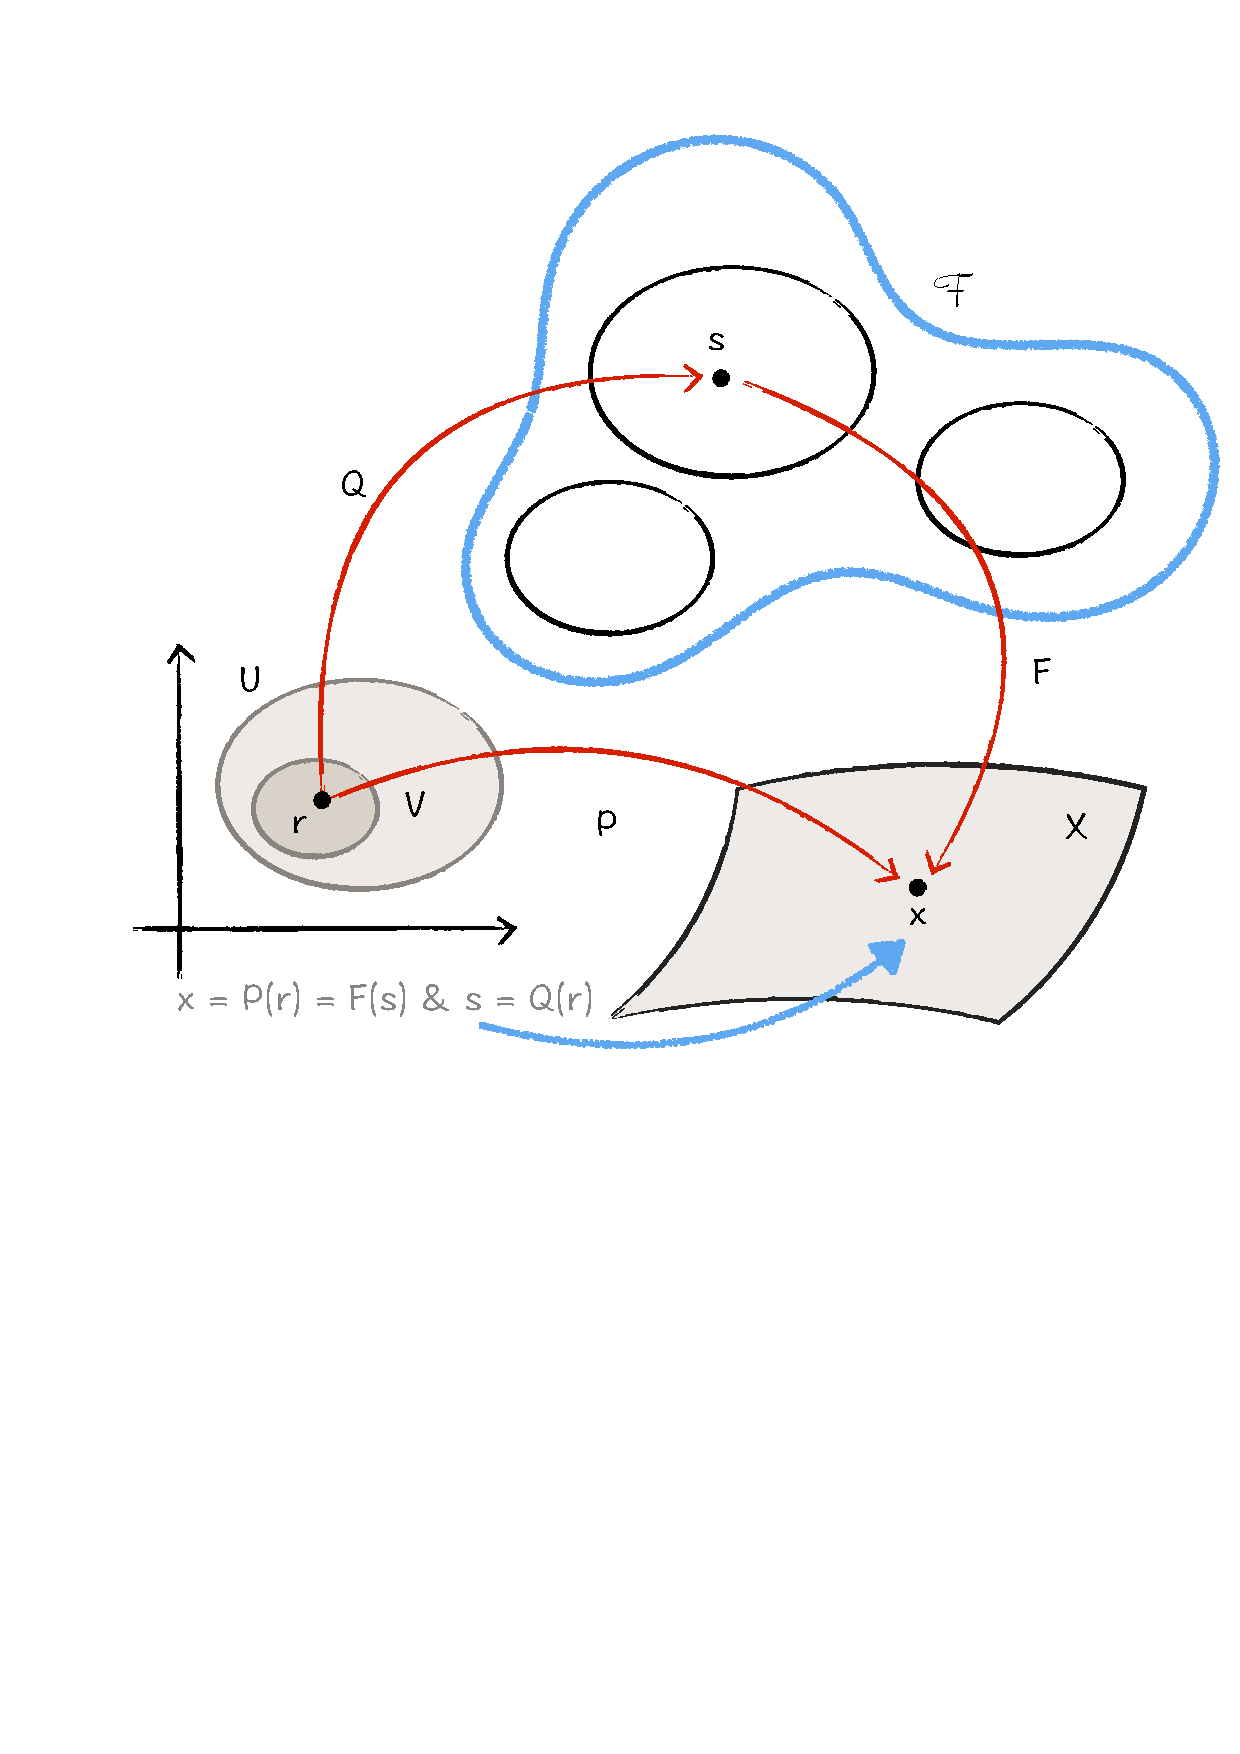
\includegraphics[width=.8\textwidth]{Figures/GenFam.pdf}
  \vspace{-.25\baselineskip}
  \caption{A generating family.}
  \label{A-generating-family}
\end{figure}
